%\documentclass[handout]{beamer}\mode<presentation>{\usetheme{AMSCesenaPurpleAndGold}}
\documentclass[presentation]{beamer}\mode<presentation>{\usetheme{AMSCesenaPurpleAndGold}}
%%%%

\usepackage{sd-lab-building-agents}
\usepackage{my-listings}
\usepackage{forloop}

\title[L5 -- Building Agents]{Building Agents from scratch}
%
\subtitle[SD]
{Distributed Systems / Laboratory\\\scriptsize Sistemi Distribuiti / Laboratorio}
%
\author[Ciatto \and Omicini]
{\emph{Giovanni Ciatto} \and Andrea Omicini\\
	\texttt{giovanni.ciatto@unibo.it} \and \texttt{andrea.omicini@unibo.it}}
%
\institute[DISI, Univ. Bologna]
{Dipartimento di Informatica -- Scienza e Ingegneria (DISI)\\\textsc{Alma Mater Studiorum} -- Universit{\`a} di Bologna a Cesena}
%
\date[A.Y. 2019/2020]{Academic Year 2019/2020}

\setbeamercovered{transparent}

\begin{document}
	
%\\\\\\\\\\\\\\\\\\\\\
\frame{\titlepage}
%\\\\\\\\\\\\\\\\\\\\\

\section{Wetting your appetite}

\begin{frame}
\frametitle{Motivation \& Lecture Goals I}

\begin{itemize}
	\item As you may have understood OOP is poorly suited for programming Distributed Systems
	
	\vfill
	
	\item This is because \alert{objects do not encapsulate control flow}
	%
	\begin{itemize}
	    \item they just encapsulate state \& behaviour (i.e. methods)
	    
	    \item any thread can invoke some object's methods, in the general case
	\end{itemize}
	
	\vfill
	
	\item This trait of OOP makes it difficult to deal with scenarios where the \alert{interaction} is the major dimension to be taken into account
    %
    \begin{itemize}
        \item[ie] those contexts where it is important to specify \alert{when} some object's behaviour or state transition should be triggered, and \alert{why}
        \item[!] defining \alert{when} to do something is as important as defining \alert{how} to do it
    \end{itemize}
    
    \vfill
    
    \item The notion of \alert{agent} has emerged, targeting this issue
    %
    \begin{itemize}
        \item it has actually been declined in several ways, depending on the context
        \item \alert{autonomy} is the most prominent feature characterising agents, regardless of the particular declination
    \end{itemize}
\end{itemize}

\end{frame}

\begin{frame}
\frametitle{Motivation \& Lecture Goals II}

\begin{itemize}
	\item In this Lab and in the next one, we borrow \alert{JADE}'s notion of agent and we try to reproduce it, step by step
	%
	\begin{itemize}
	    \item[!] \alert{before next lab}, you are kindly invited to recall JADE's agents and behaviours functioning
	\end{itemize}
	
	\vfill
	
	\item We here consider an agent as an object (in the OOP sense) with its own \alert{logical} control flow
	
	\vfill
	
	\item Differently from what we did so far, we won't explicitly use \alert{threads}
	
	\vfill
	
	\item Our agents will share the same \texttt{ExecutorService}, when running within the same JVM
	%
	\begin{itemize}
	    \item this will provide our agents with great \alert{scalabilty \& lightweightness}
	\end{itemize}
\end{itemize}

\end{frame}

\begin{frame}
\frametitle{Motivation \& Lecture Goals III}

\begin{itemize}
	\item In this Lab we will simply focus on designing a way for objects to encapsulate control flow
	
	\vfill
	
	\item In the next Lab we will focus on endowing agents with \emph{multiple} \alert{logical} control flow
	%
	\begin{itemize}
	    \item i.e. something similar to JADE's behaviours
	\end{itemize}
	
	\vfill
	
	\item Finally, the future Labs will be devoted to opening our agent-based to \alert{distribution}
	
\end{itemize}

\end{frame}

\subsection{About the practical activities}

\begin{frame}
\frametitle{Lab 5 Repository on GitLab}

	\begin{itemize}
		\item Examples and exercises described in this lecture are provided by means of the following GitLab repository:
		%
		\begin{center}
			\url{https://gitlab.com/pika-lab/courses/ds/aa1920/lab-05}
		\end{center}
		
		\vfill
		
		\item Clone it on your machine using Git
		%
		\begin{itemize}
		    \item[\$] \texttt{git clone \textit{<repo URL>}}
		\end{itemize}
		
		\vfill
		
		\item Even if a minimal environment simply relying on a text editor + Gradle is sufficient for this lab, we kindly suggest to import the cloned repository into some IDE, e.g. IntelliJ Idea or Eclipse
		%
		%
		\begin{itemize}
		    \item in case of problems in importing the project on IntelliJ, try to downgrade the gradle wrapper
		    %
		    \item[\$] \texttt{./gradlew wrapper \alert{--gradle-version \textit{4.8.1}}}
		\end{itemize}
		
		\vfill
		
		\item In order to be able to submit your exercises, please ensure you requested access to the \href{https://gitlab.com/pika-lab/courses/ds/aa1920}{GitLab group of the course}
	\end{itemize}

\end{frame}

\section{Towards JADE-like MAS}

\subsection{Overview}

\begin{frame}
\frametitle{Overview}

	\begin{block}{MAS}
	    We consider a MAS to be composed by a number of agents \alert{interacting} within an environment
	\end{block}
	
	\vfill
	
	\begin{block}{Agent}
	    We consider an Agent as an object (data + behaviour) coming with its own \alert{logical} control flow
	\end{block}
	%
	\begin{itemize}
	    \item[!] we prefer to avoid the \alert{1-agent-1-thread} situation, to prevent scalability issues
	\end{itemize}
	
	\vfill
	
	\begin{block}{Environment}
	    We consider an Environment as a container of agents, exposing \alert{shared} facilities aimed at \alert{supporting} the agents' interaction
	\end{block}
	%
	\begin{itemize}
	    \item[!] we will rely on shared \alert{\texttt{TextualSpace}s} for such purpose
	\end{itemize}
\end{frame}

\subsection{Environment}

\begin{frame}[allowframebreaks]{Environment -- Interface}
    
    \lstinputlisting{code/Environment.java}
    
\end{frame}

\begin{frame}{Environment -- Design Rationale}
    
    \begin{itemize}
        \item All agents from within the same environment \alert{share} the same \texttt{ExecutorService}
        %
        \begin{itemize}
            \item we call it \alert{engine} since it is responsible for all computations actually occurring within the system
        \end{itemize}
        
        \vfill
        
        \item Shared \texttt{TextualSpace}s are available \alert{to all agents} within the environment
        %
        \begin{itemize}
            \item each agent can access each tuple space through its \alert{name}
            \item each possible name is \alert{virtually} bound to a tuple space
            %
            \begin{itemize}
                \item instances of tuple spaces are \alert{actually created} upon first usage
            \end{itemize}
        \end{itemize}
        
        \vfill
        
        \item Conventions on how to use tuple space names or how to structure tuples is up to the agents
        
        \vfill
        
        \item Agents can either
        %
        \begin{itemize}
            \item be created outside the environment and then join it thorugh \alert{registration}
            %
            \item be created as part of the environment
        \end{itemize}
        
    \end{itemize}
    
\end{frame}

\begin{frame}[allowframebreaks]{Environment -- Implementations}
    
    \begin{block}{\texttt{sd.lab.agency.impl.\textit{AbstractEnvironment}}}
        Provides common facilities for agents' initialisation and registration
    \end{block}
    
    \vfill
    
    \begin{exampleblock}{\texttt{sd.lab.agency.impl.\textit{LocalEnvironment}}}
        Extends the \texttt{AbstractEnvironment} in such a way that the \texttt{TextualSpace}s created by \texttt{getTextualSpace(String)} are \alert{local} and backed by the same \texttt{ExecutorService} returned by \texttt{getEngine()}
    \end{exampleblock}
    
    \vfill
    
    \begin{alertblock}{(Spoiler Alert) \textbf{Distributed} Environment}
        Hides distribution behind the same interfaces used for the local implementation
    \end{alertblock}
    
\end{frame}


\subsection{Agent}

\begin{frame}[allowframebreaks]{Agent -- Interface}
    
    \lstinputlisting{code/Agent.java}
    
    \lstinputlisting{code/AndThen.java}
    
\end{frame}

\begin{frame}{Agent -- Naming}

For practical reasons, agents have two names:
%
\vfill
%
\begin{description}
    \item[local name] can be any string, but it must be \alert{unique} within the environment the agent is situated into
    
    \vfill
    
    \item[full name] = local name + environment name
    
\end{description}

\end{frame}

\begin{frame}[allowframebreaks]{Agent -- Rationale}
    
    % \begin{block}{Agent VS User perspectives}
    %     The functioning of agents can be described and understood according to two different perspectives:
        
    % \end{block}
    
    Expected functioning of all objects of type \alert{\texttt{Agent}}:
    %
    \vspace{.5cm}
    %
    \begin{itemize}
        \item the agent is created by some other entity as an ordinary Java object
        
        \vspace{.5cm}
        
        \item the agent may be started from outside by means of the \texttt{Agent::\alert{start()}} method 
        %
        \begin{itemize}
            \item this is the only tolerated exception to control encapsulation
        \end{itemize}
        
        \vspace{.5cm}
        
        \item once started, the following things should happen:
        %
        \begin{enumerate}
            \item the \texttt{Agent::\alert{onBegin()}} callback is executed \alert{just once}
            
            \item \alert{after} that, the \texttt{Agent::\alert{onRun()}} method is executed an \alert{unlimited} amount of times, sequentially
    
            \item the sequence of executions of \texttt{onRun()} can only be interrupted by the agent itself by calling the \texttt{Agent::\alert{stop()}} method inside its \texttt{onBegin()} or \texttt{onRun()} callbacks
        \end{enumerate}
        
        \framebreak
        
        % \item if the agent calls its \texttt{Agent::\alert{pause()}} method, the sequence of \texttt{onRun()} is interrupted as well
        
        % \vspace{.5cm}
        
        % \item however, if some external entity calls the 
        % \texttt{Agent::\alert{resume()}} method on a paused agents, the sequence of \texttt{onRun()} is resumed \alert{from where it had been interrupted}
        
        % \vspace{.5cm}
        
        % \item if the agent calls its \texttt{Agent::\alert{restart()}} method, the sequence of \texttt{onRun()} is restarted---and the \texttt{onBegin()} method is executed one more time
        
        % \vspace{.5cm}
        
        % \item finally, external entities can wait for an agent's termination by means of the \texttt{Agent::\alert{await()}} method and its overloads
        
        % \framebreak
        
        % \item in any scenario, if some \alert{uncaught exception} is thrown within the \texttt{onBegin()} or \texttt{onRun()} methods, the \texttt{Agent::\alert{onUncaughtError(Exception)}} callback is called
        
        % \vspace{.5cm}
        
        % \item what happens next depends on the value returned by the \texttt{onUncaughtError(Exception)} callback, which is of type \alert{\texttt{AndThen}}
        % %
        % \begin{description}
        %     \item[\texttt{CONTINUE}] | the exception is ignored and the sequence of \texttt{onRun()} is unaffected
            
        %     \item[\texttt{PAUSE}] | the sequence of \texttt{onRun()} is paused
        % \end{description}
        
        \item after that, the agent \alert{terminates}---which means that all entities which possibly invoked the \texttt{Agent::\alert{await()}} method, can now resume their computation
        
        \vspace{.3cm}
        
        \item within its \texttt{onBegin()}, \texttt{onRun()}, or \texttt{onEnd()} methods, an agent can call the following methods affecting its own control flow and, in particular, the sequence of \texttt{on*()} methods executions:
        %
        \begin{description}\small
            \item[\texttt{stop()}] states that the next method to be executed should be \texttt{onEnd()}
            
            \item[\texttt{restart()}] states that the next method to be executed should be \texttt{onBegin()}
            
            \item[\texttt{pause()}] states that no method should be executed next, until \texttt{resume()} is called
            
            \item[\texttt{resume()}] states that the sequence of \texttt{on*()} methods executions should be resumed starting from where it was interrupted by the \texttt{pause()}
        \end{description}
        
        \framebreak
        
        \item \alert{no uncaught exception} should be able to break the aforementioned workflow
        
        \vspace{.3cm}
        
        \item to this end, \texttt{Agent::\alert{onUncaughtError(Exception)}} method is executed for each excpetion which is not caught within the \texttt{onBegin()}, \texttt{onRun()}, or \texttt{onEnd()} methods
        
        \vspace{.3cm}
        
        \item the \texttt{onUncaughtError(Exception)} method returns an object of type \texttt{AndThen} stating what should happen next:
        %
        \begin{itemize}
            \item in case \texttt{AndThen.\alert{CONTINUE}} is returned, the aforementioned workflow continues as if the exception didn't occurred
            
            \item in case \texttt{AndThen.\alert{STOP}} is returned, the aforementioned workflow is interrupted as if \texttt{stop()} was invoked
            
            \item in case \texttt{AndThen.\alert{PAUSE}} is returned, the aforementioned workflow is interrupted as if \texttt{pause()} was invoked
            
            \item in case \texttt{AndThen.\alert{RESTART}} is returned, the aforementioned workflow is restarted as if \texttt{restart()} was invoked
        \end{itemize}
        
        
    \end{itemize}
    
    
\end{frame}

\subsection{Examples of valid scenarios}

\begin{frame}{Normal Flow}\centering
    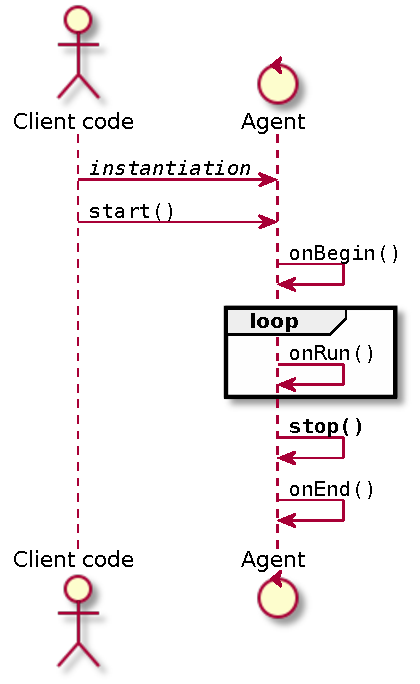
\includegraphics[height=.8\textheight]{img/normal-flow.pdf}
\end{frame}

\begin{frame}{Pause and Resume}\centering
    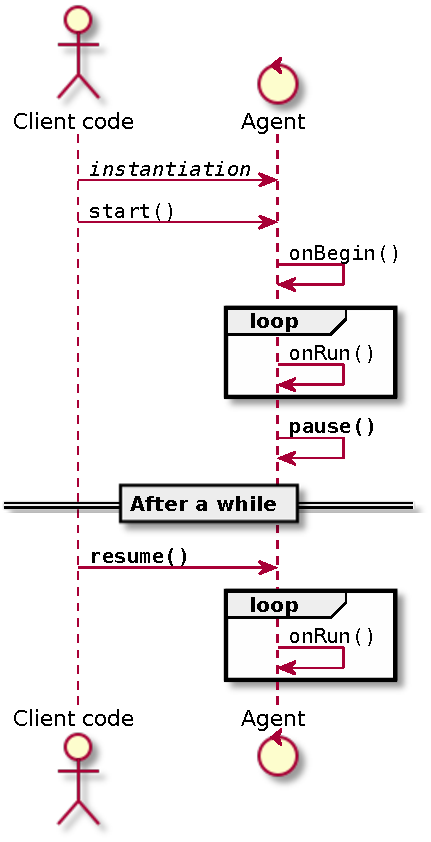
\includegraphics[height=.8\textheight]{img/paused-flow.pdf}
\end{frame}

\begin{frame}{Uncaught Exceptions}\centering
    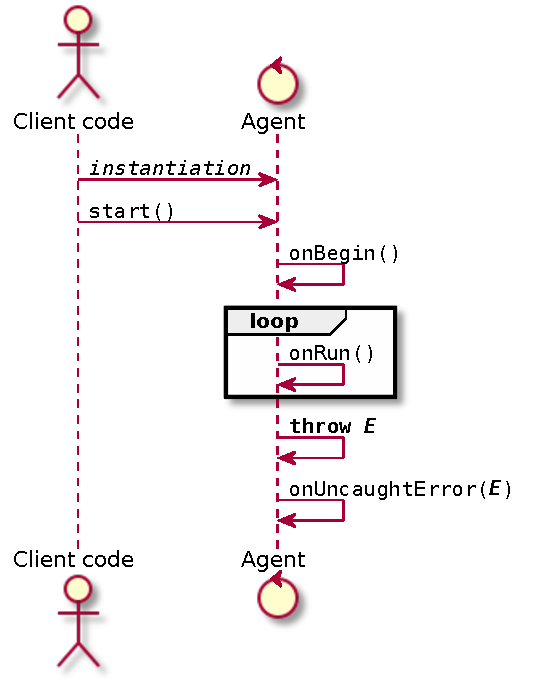
\includegraphics[height=.8\textheight]{img/exceptional-flow-1.pdf}
    \hspace{.5cm}
    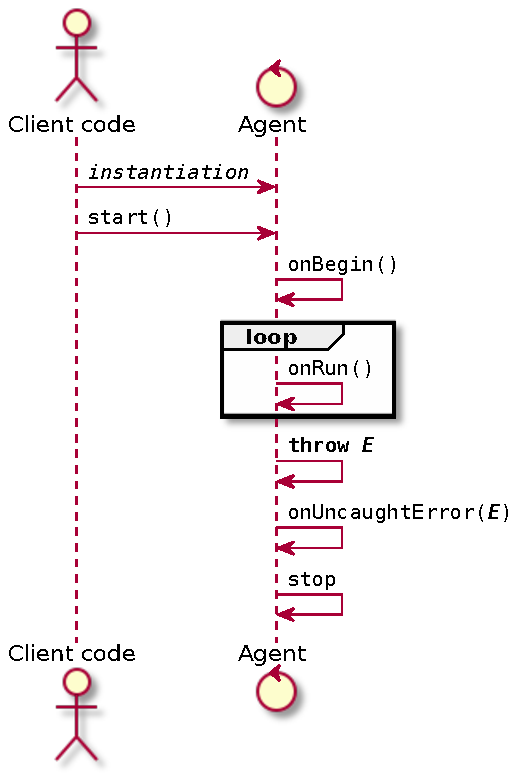
\includegraphics[height=.8\textheight]{img/exceptional-flow-2.pdf}
\end{frame}

\begin{frame}{Restart}\centering
    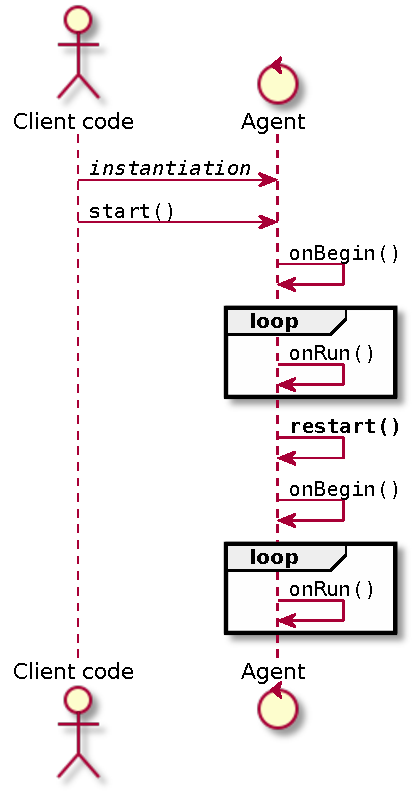
\includegraphics[height=.8\textheight]{img/restarted-flow.pdf}
\end{frame}

\begin{frame}{UsageExample}\centering
    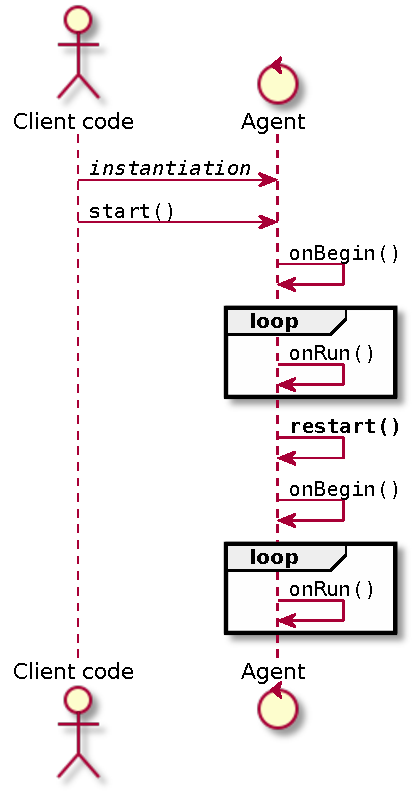
\includegraphics[height=.8\textheight]{img/restarted-flow.pdf}
\end{frame}

\subsection{Why is this cool}

\begin{frame}{What's the purpose of this architecture?}

\begin{itemize}
    \item This is a relatively compact architecture that will be the basis of several mechanisms
    
    \vfill
    
    \item In particular, it enables several agents to compute and interact in a \alert{non-blocking} way
    
    \vfill
    
    \item For instance in the next slide, 3 agents sharing the same \alert{single-threaded} executor service, are capable to perform multiple \alert{suspensive} operations without the whole system getting stuck
\end{itemize}

\end{frame}

\begin{frame}[allowframebreaks]{Example}
    \lstinputlisting{code/Sender.java}
    %
    \hint{Consider reasing the documentation for \href{https://docs.oracle.com/en/java/javase/12/docs/api/java.base/java/util/concurrent/CompletableFuture.html}{\texttt{CompletableFuture::\alert{thenApplyAsync}}}}
    
    \lstinputlisting{code/Receiver.java}
    
    \lstinputlisting{code/SenderReceiver.java}
    
    
    %
    % \begin{columns}
    %     \begin{column}{.49\linewidth}
        
    %     \end{column}
    %     \hfill
    %     \begin{column}{.49\linewidth}
        
    %     \end{column}
    % \end{columns}
\end{frame}

\subsection{Agent FSA}

\begin{frame}[allowframebreaks]{Agents' Finite State Automaton (FSA)}

    \begin{itemize}
        \item The agents' functioning just described can be modelled through a FSA
        
        \vspace{0.3cm}
        
        \item Such FSA would be composed by $5+1$ states:
        %
        \begin{description}
            \item[CREATED] | the agent has been instantiated but not yet started
            
            \item[STARTED] | after the \texttt{start()} method has been called
            
            \item[RUNNING] | after the \texttt{onBegin()} callback has been executed
            
            \item[PAUSED] | after the \texttt{pause()} method has been called
            
            \item[STOPPED] | after the \texttt{stop()} method has been called
            
            \item[terminated] | after the \texttt{onStop()} callback has been executed
        \end{description}
        
        \framebreak
        
        \item State transitions imply consuming some value of type \texttt{\alert{AndThen}} and executing a callback
        
        \vspace{.3cm}
        
        \item State transition are usually provoked by invocations of the \alert{control methods}
        %
        \begin{itemize}
            \item[ie] the \texttt{start()}, \texttt{stop()}, \texttt{restart()}, \texttt{pause()}, or \texttt{resume()} methods
        \end{itemize}
        
        \vspace{.3cm}
        
        \item We say such methods \alert{feed} input values (i.e. instances of \texttt{AndThen}) to the FSA
        
        \vspace{.3cm}
        
        \item If no \alert{control method} is called within a callback, \texttt{AndThen.\alert{CONTINUE}} is feeded to the FSA, by default
    \end{itemize}
    
    \framebreak
    
    \begin{center}
        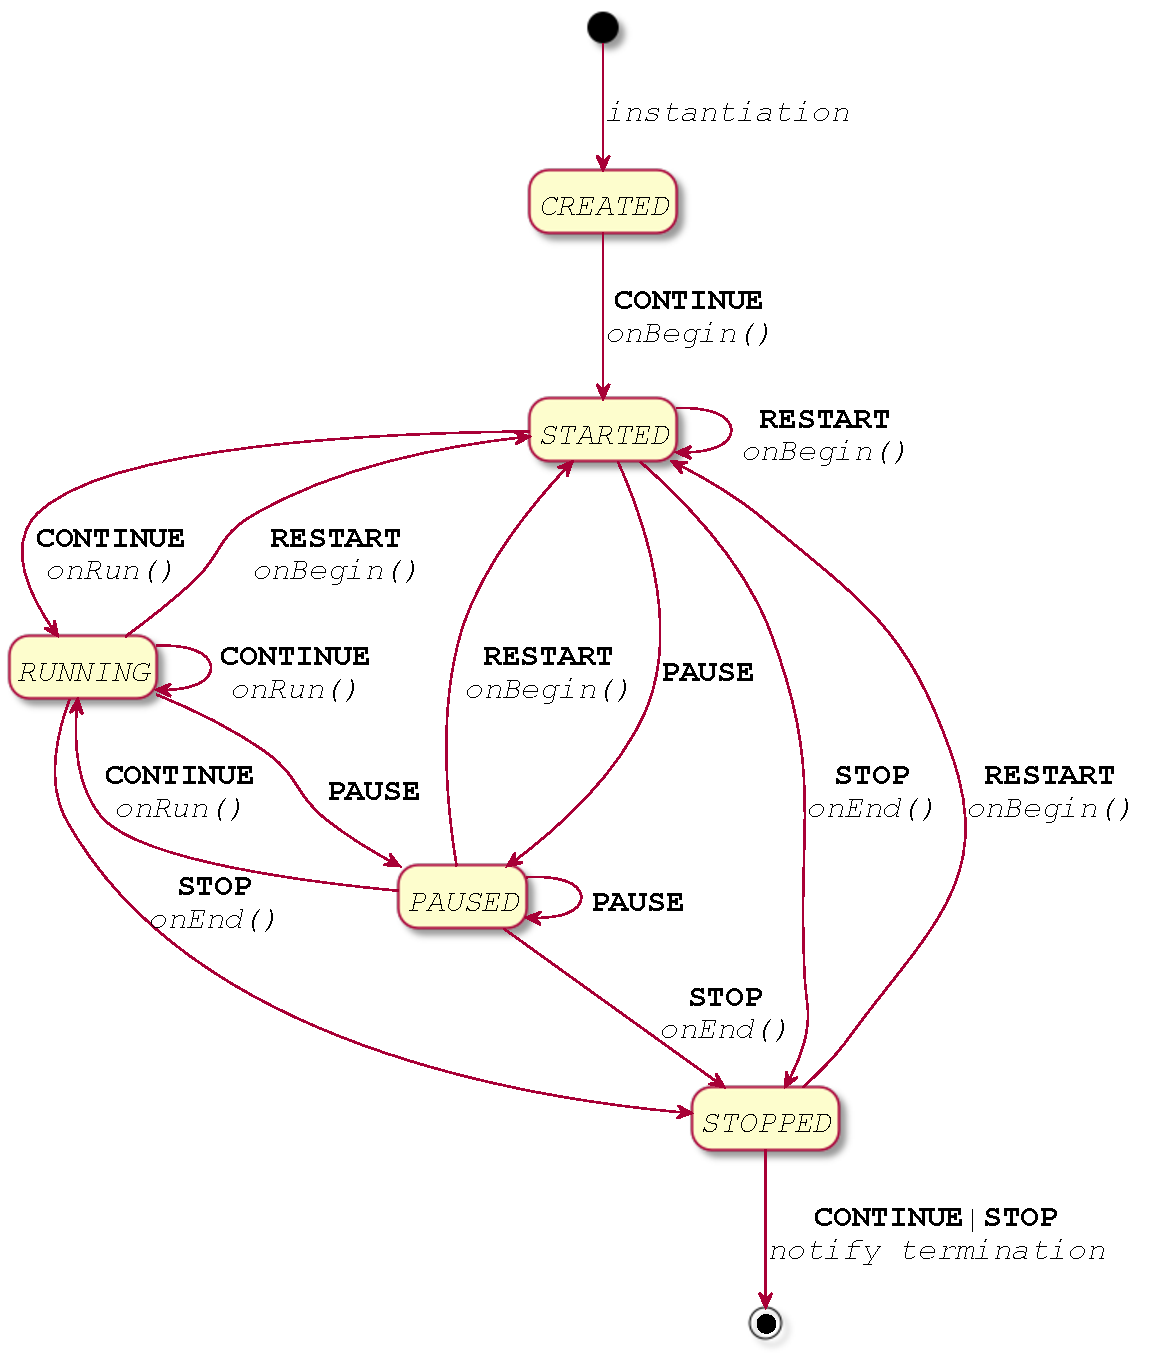
\includegraphics[height=.9\textheight]{img/fsa.pdf}
    \end{center}
    
\end{frame}

\section{Exercises}

\subsection{Implementing the FSA}

\begin{frame}[allowframebreaks]{Exercise 5-1 -- Implementing \texttt{BaseAgent}}
    Consider the \texttt{sd.lab.agency.impl.\alert{BaseAgent}} class:
    %
    \lstinputlisting{code/BaseAgent.java}
    
    \framebreak
    
    \begin{block}{TODO}
        Complete the implementation of the following methods:
        %
        \begin{itemize}
            \item \texttt{BaseAgent::\alert{doStateTransitionFrom\textit{Created}}}
            
            \item \texttt{BaseAgent::\alert{doStateTransitionFrom\textit{Started}}}
            
            \item \texttt{BaseAgent::\alert{doStateTransitionFrom\textit{Running}}}
            
            \item \texttt{BaseAgent::\alert{doStateTransitionFrom\textit{Paused}}}
            
            \item \texttt{BaseAgent::\alert{doStateTransitionFrom\textit{Stopped}}} 
            
            \item \texttt{BaseAgent::\alert{doBegin}}, and  \texttt{BaseAgent::\alert{begin}}
            
            \item \texttt{BaseAgent::\alert{doRun}}, and \texttt{BaseAgent::\alert{run}}
            
            \item \texttt{BaseAgent::\alert{doEnd}}, and \texttt{BaseAgent::\alert{end}}
        \end{itemize}
        %
        in such a way that all tests in \texttt{sd.lab.agency.\alert{TestAgent}} are satisfied
    \end{block}
\end{frame}

\subsection{A simple ping-ping system}

\begin{frame}[allowframebreaks]{Exercise 5-2 -- Implementing ping-pong}

\begin{block}{TODO}
    \begin{itemize}
        \item Complete the implementation of \texttt{\alert{PongAgent}}
        
        \item In such a way that all tests in \texttt{sd.lab.agency.\alert{TestPingPong}} are satisfied
    \end{itemize}
\end{block}

\begin{alertblock}{Question time}
    \begin{itemize}
        \item Can you see why suspensive operations are non-blocking in our architecture?
        
        \item Can you see where our architecture falls short?
    \end{itemize}
\end{alertblock}

\end{frame}

%===============================================================================
\section*{}
%===============================================================================

%\\\\\\\\\\\\\\\\\\\\\
\frame{\titlepage}
%\\\\\\\\\\\\\\\\\\\\\

%%===============================================================================
%\section*{\refname}
%%===============================================================================
%
%%\\\\\\\\\\\\\\\\\\\\\
%%%%%
%%\begin{frame}[t,allowframebreaks]\scriptsize
%\begin{frame}[c]\footnotesize
%\frametitle{\refname}
%\bibliographystyle{apalike}
%\bibliography{sd-lab-building-linda}
%\end{frame}
%%\\\\\\\\\\\\\\\\\\\\\

%%%%%%%%%%%%%%%%%%%%%%%%%%%%%%%%%%%%%%%%%%%%%%%%%%%%%%%%%%%%%%%%%%%%%%%%%%%%%%%
\end{document}
%%%%%%%%%%%%%%%%%%%%%%%%%%%%%%%%%%%%%%%%%%%%%%%%%%%%%%%%%%%%%%%%%%%%%%%%%%%%%%%%

